\chapter{Orthogonality}\label{chap:ortho}
In this chapter, we will begin to develop the geometric framework of lengths and angles through the lens of linear algebra. While the notions of affine geometry were introduced earlier in \chapref{chap:vectors}, this chapter will develop the notions of Euclidean geometry. As such, this geometric development will not be entirely possible for the finite fields $\Z_p$ we have often considered, although some notion of orthogonality are available for general fields. In this chapter the only fields $F$ we will consider for scalars will be $\R$ and $\C$. \\

\begin{center}
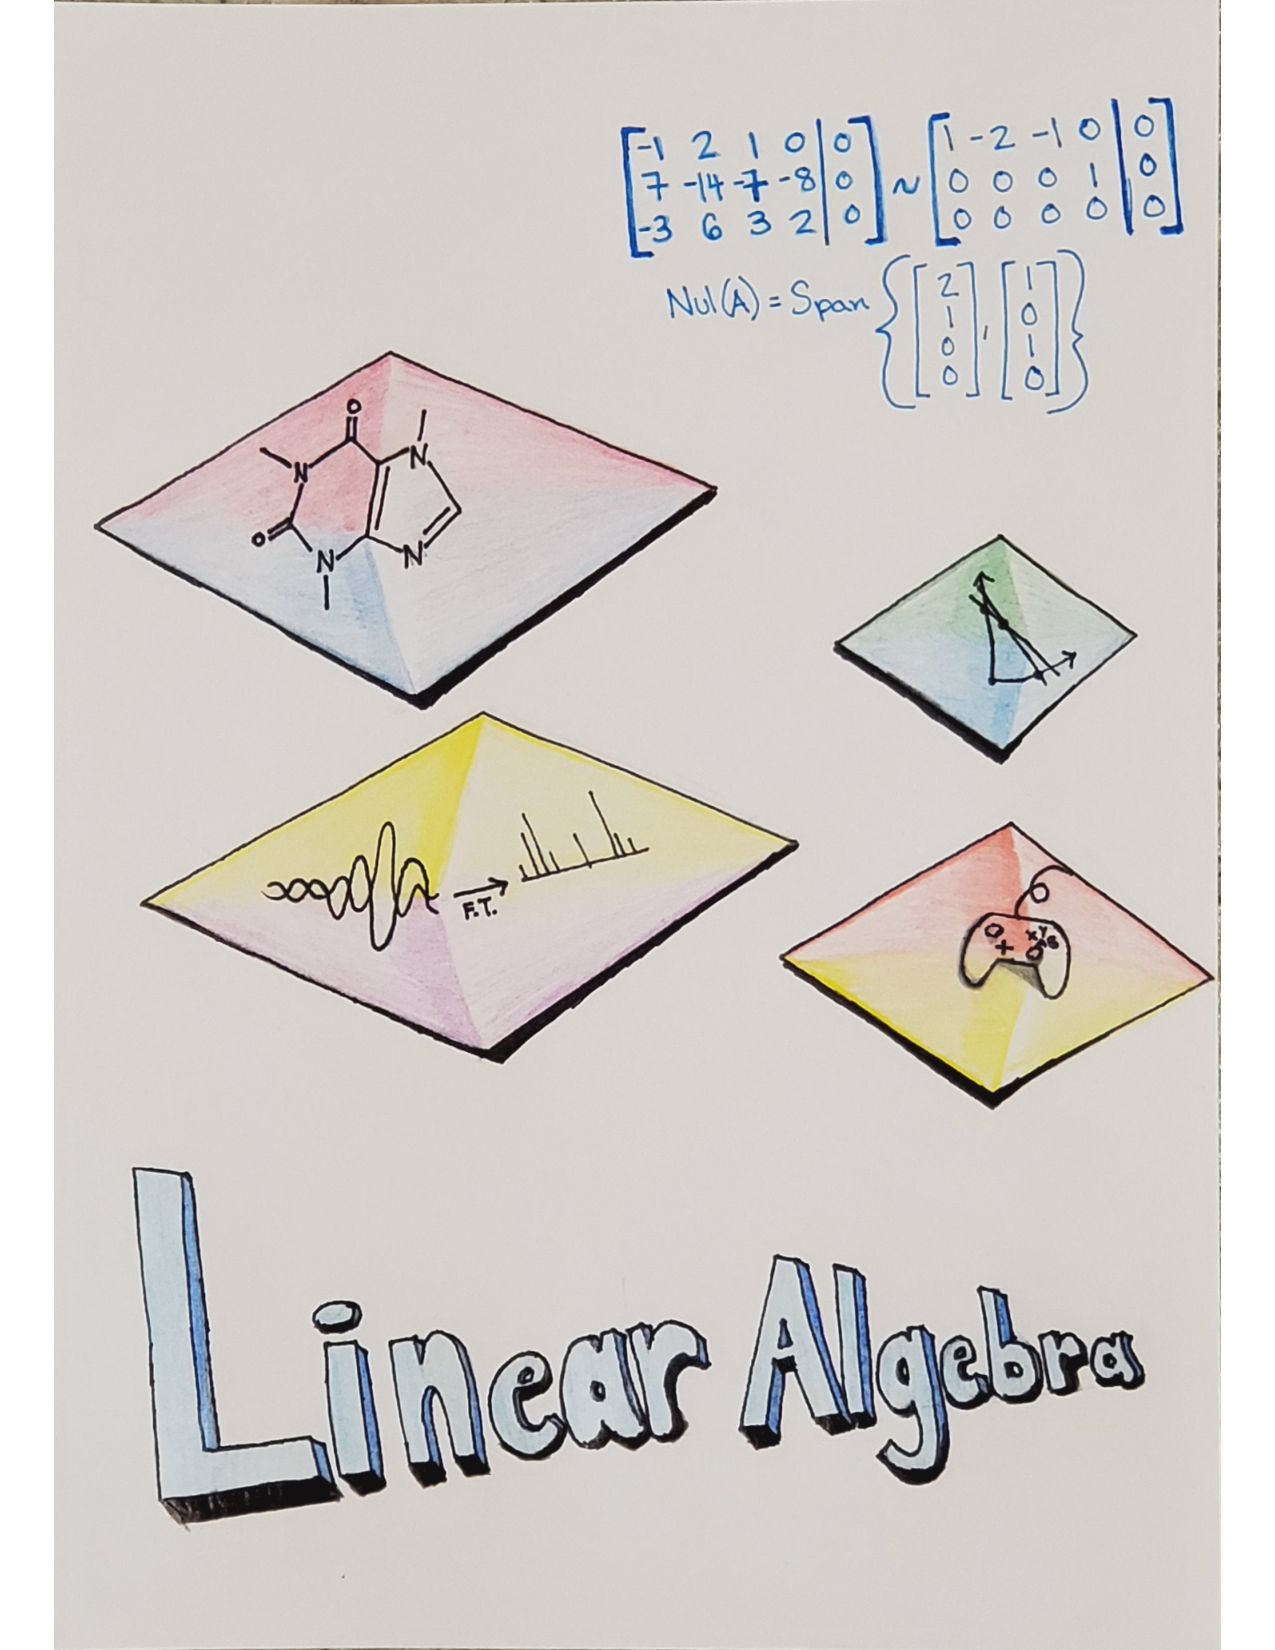
\includegraphics[scale=0.75, trim = 40 255 29 45, clip]{Chapter4/images/Chapter4cover.pdf}%Mariah Clayson
\end{center}
%{\vspace{-10 pt}\hfill\footnotesize (Drawing contributed by Mariah Clayson)}\\ %The main focus of the design is the four basic shapes in the center, representing the Fundamental Theorem of Linear Algebra. Inside of each of the parallelograms is a representation of real life linear algebra applications. Starting with the top left, this caffeine molecule is to represent the use of linear algebra in balancing chemical equations, solving for concentrations in systemic treatments of equilibrium, and solving for absorbance values particularly in UV-vis when several different molecules are in the solution. The bottom left picture is a representation of a Fourier Transform which is typically used to convert a time domain to a frequency domain, especially in NMR (Nuclear Magnetic Resonance spectroscopy) which is used to identify compounds in chemical labs. The top right figure is a representation of linear programming that can be used to find optimal solutions in a variety of settings. The bottom right picture is meant to represent video games and 3D graphics in general as they are a projection of three dimensional components onto a two-dimensional screen. The top most component of the cover art is an example of matrices being used to calculate the null space. The title itself is also meant to be a ``3D” image that represents linear algebra’s usefulness in this area.

\pagebreak  